\documentclass[titlepage]{article}

\usepackage{graphicx}
\usepackage{subcaption}
\graphicspath{ {./images/} }
\usepackage{hyperref}
\usepackage{pdfpages}
\usepackage{cite}
\usepackage{url}


\newcommand{\figref}[1]{Figure ~\ref{fig:#1}}

\title{Title}

\author{
	Jake Hermle\\ \emph{Civil Engineering} \and
	Nakul Joshi\\ \emph{Computer Engineering} \and
	John Lally\\ \emph{Mechanical Engineering}\and
	Christine Noh\\ \emph{International Relations}
}

%ADD LETTERS
%ADD RESUMES (pdfpages class)

\begin{document}
\maketitle

\begin{abstract}

\end{abstract}

\tableofcontents
\newpage
\listoffigures
\newpage
\listoftables
\newpage



\section{Introduction}

Community Health Councils (CHC) is producing a report for the City of Los Angeles that recommends and details guidelines for complete streets design to be included in the Mobility Element of the city’s General Plan. This CHC report will be describing various best practices that can be implemented so that LA streets better adhere to the principles of complete streets. The following report details eight specific best practices that CHC may implement in their report to the City of Los Angeles. For each best practice, a general description is provided, as well as a discussion of its impact and cost. Additionally, each practice was evaluated based on its cost, impact, and ease of implementation to determine whether it is worth recommending as a design guideline in the Mobility Element. A usability index was created to more quantitatively evaluate these practices, and allowed for better comparison between them. In addition to complete street design, this report is also mindful of CHC’s overarching goals of improving health in South LA.

\newpage

\section{Best Practices}
	\subsection{Chokers} Chokers are curb extensions at midblock locations that narrow a street by ultimately creating wider sidewalks. They are also known as safe crosses when marked as crosswalks. Chokers can be made by widening one side of the curb or by bringing both curbs in, giving it the “pinch point” along the street (See \figref{choker}). The main purpose of chokers is to decrease speed of incoming vehicles at a mid-point along the streets, create a seamless transition between a commercial and a residential area, and to narrow exceedingly wide intersections \cite{walking-info-chokers}.

\begin{figure}[h]
\centering
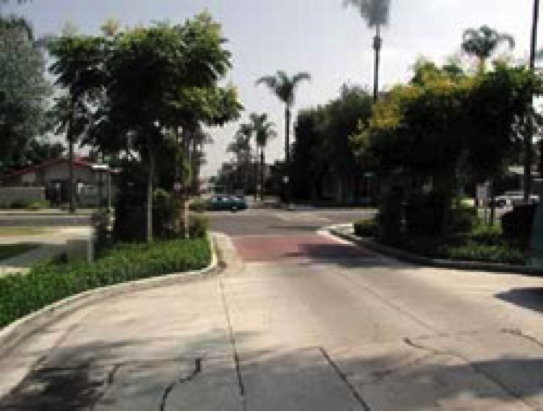
\includegraphics[scale=1]{choker.png}
\caption[Choker]{This choker requires drivers to yield upon entering}\label{fig:choker}
\end{figure}

Two-lane chokers (See \figref{two-lane-choker}) leave two lanes in the street cross section narrower than the width of a normal cross section, while one-lane chokers narrow the width to allow travel in only one direction at a time. These chokers are effective for areas with substantial speed problems and streets with minimum or no parking on-site.

\begin{figure}
\centering
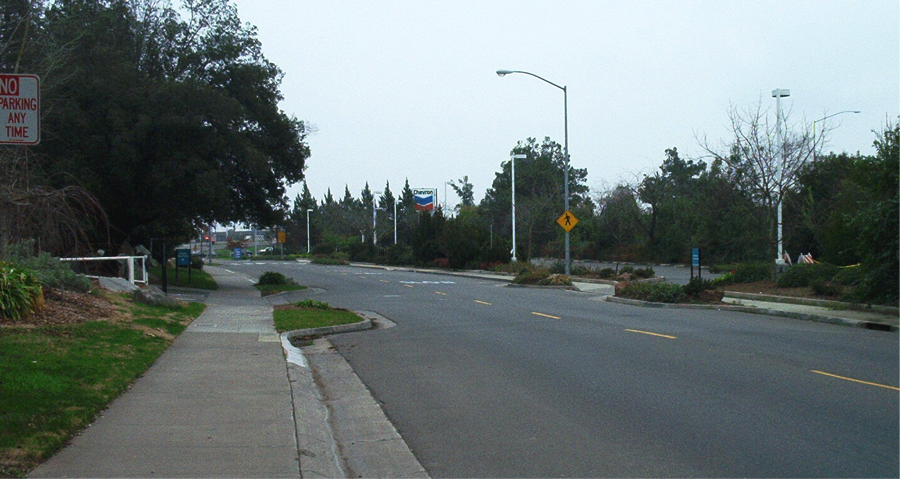
\includegraphics[scale=1]{two-lane-choker.png}
\caption{Two-Lane Chokers}\label{fig:two-lane-choker}
\end{figure}

\subsubsection{Advantages and Disadvantages}

The various advantages of chokers are:\begin{itemize}
\item ability to reduce both speed and volume significantly
\item easily negotiable by large vehicles (for example, fire trucks)
\item improving aesthetic value when well designed
\end{itemize}

The disadvantages include:\begin{itemize}
\item Eliminates on-street parking
\item Requires bicyclists to briefly merge with vehicular traffic
\item Absence of vertical or horizontal deflation limiting the effect of chokers on vehicle speed.
\end{itemize}

\subsubsection{Effectiveness}

Chokers can ultimately increase the visibility of pedestrians as well as to reduce pedestrian crossing width, while the speed of vehicles is reduced by 4 percent on average for two-lane chokers and 14 percent on average for one-lane chokers \cite{ite}. Also since chokers work well with speed humps, speed tables, and raised intersections, (See \figref{speed-hump}) it can be created in many sites with no extreme difficulty.

\begin{figure}
\centering
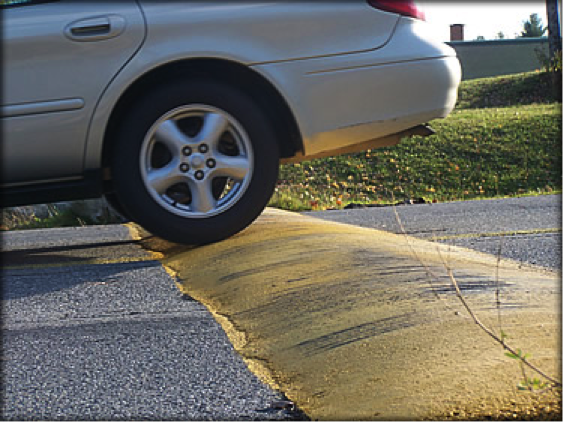
\includegraphics[scale=1]{speed-hump.png}
\caption{Speed Hump}\label{fig:speed-hump}
\end{figure}

\subsubsection{Cost and Considerations}

Factors to consider when creating chokers are to consult with the local fire and sanitation department before setting minimum width and to double check to make sure that the bicyclist safety and mobility are not diminished. Also when reducing two-lane street to one lane, the width of the travel way should not be wide enough for 2 cars to pass at the same time. This equals to the travel way not being wider than 4.9 meter, or 16 to 17 feet; by doing so, the effectiveness of the chocker is maximized \cite{walking-info-chokers}. The cost to create chokers varies depending on the site and landscape but most are along the lines of \$5,000 to \$20,000 (drainage representing a significant amount).
	\subsection{Curb Radius}
	Curb radius is a traffic calming technique in which the grid of intersecting streets is reshaped and the radius of the curb is significantly reduced. As you can see in \figref{large-radius}, a large curb radius will enable vehicles to go around corners faster while in \figref{small-radius}, a smaller curb radius will slow vehicles down when turning into the corner.

\begin{figure}[h]
\centering
\begin{subfigure}[b]{0.4\textwidth}
	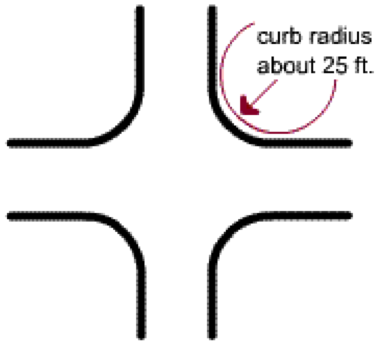
\includegraphics[width=\textwidth]{large-radius.png}
	\caption{Large Curb Radius}\label{fig:large-radius}
\end{subfigure}
\begin{subfigure}[b]{0.4\textwidth}
	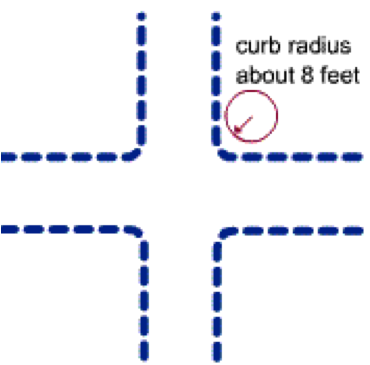
\includegraphics[width=\textwidth]{small-radius.png}
	\caption{Small Curb Radius}\label{fig:small-radius}
\end{subfigure}
\end{figure}

        The purpose of curb radii is to slow vehicles down by enabling them to make smaller turns, which ultimately reduces the risk of pedestrians being struck by vehicles when turning into a corner. Also, small curve radii can create safer intersections, improve the visibility between drivers and pedestrians, and lead to improved signal timing. By reducing the curb radii, not only will it slow down vehicles when turning, but it will also shorten the distance and time it takes for pedestrians to cross the street by nearly half of what it used to be (See Table ~\ref{table:cross-time-vs-radius} and Figures ~\ref{fig:radius-change} and ~\ref{fig:cross-time-vs-radius}).
        
\begin{figure}[h]
\centering
	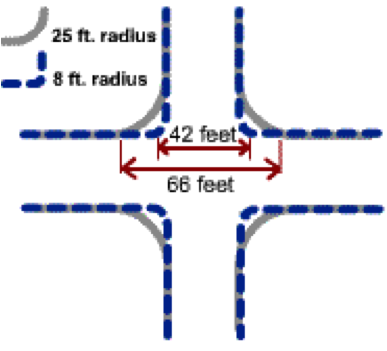
\includegraphics[scale=1]{radius-change.png}
	\caption[Effect of changing curb radius]{Change in Distance from 25ft. Radius to 8ft. Radius}\label{fig:radius-change}
\end{figure}

\begin{table}[h]
\centering
    \begin{tabular}{cc}
    Curb Radius (feet) & Average crossing time (seconds) \\ \hline
    10                 & \phantom{0}7.9                             \\
    15                 & \phantom{0}9.8                             \\
    25                 & 14.1                            \\
    \end{tabular}
\end{table}

\begin{figure}[h]
\centering
	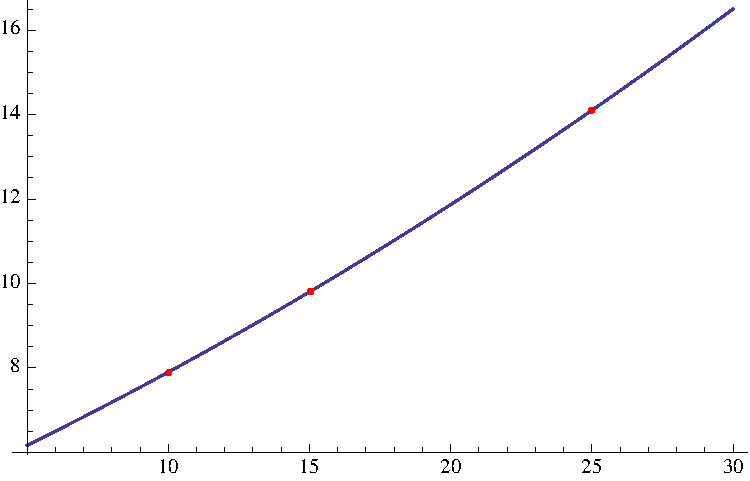
\includegraphics[scale=0.5]{cross-time-vs-radius.pdf}
	\caption[Plot of crossing times against curve radii]{A plot of the data from Table ~\ref{table:cross-time-vs-radius}}\label{fig:cross-time-vs-radius}
\end{figure}

        When streets have a large curb radius, motorists can make turns at relatively high speeds that decrease pedestrian safety. By contrast, 90-degree intersections and corners with tight curb radii tend to slow motorists down and therefore increase pedestrian safety. Motorists turning right at high speed can cut off bicyclists/pedestrians traveling straight on the arterial street. In addition, pedestrians crossing the residential street adjacent to the arterial may not expect high-speed turning traffic, or they may have their backs facing the turning cars as you can see in ~\ref{fig:back-against-car}

\begin{figure}
\centering
	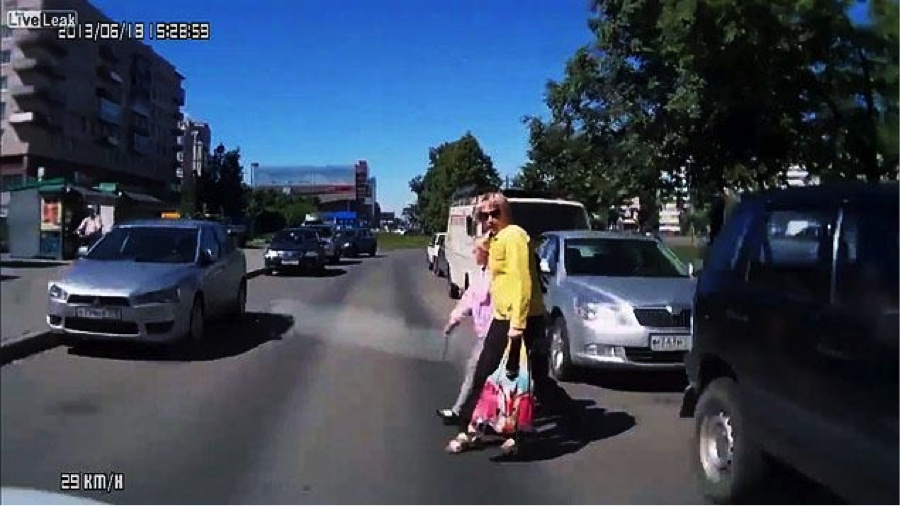
\includegraphics[width=0.5\textwidth]{back-against-car.png}
	\caption{Pedestrian Facing Back Against the Car}\label{fig:back-against-car}
\end{figure}

The cost of reconstructing tighter turning radii is in between \$5,000 to \$40,000 per corner depending on the site locations/conditions. When considering curb radii, it is important to note that in order for it to be effective, the design should meet the needs of the design vehicles with consideration for nearby land uses and prevalence of roadway users. So if there are high volumes of large vehicles making turns in a given location, a poorly designed curb radius could potentially cause the vehicles to drive over the curb and onto the sidewalk endangering pedestrians. In addition, you should always accommodate emergency vehicles, as well as school buses, and public maintenance vehicles when designing curb radii\cite{walking-info-curb}.


There is no magic number for the appropriate curb radius because it differs case by case depending on where it is located (See \figref{location-depend}). The length of the curb radius that should be used wherever possible is 5 to 10 feet, whereas an effective radius for urban streets with high volumes of pedestrians is 15 to 20 ft. For arterial streets with a substantial volume of turning buses/trucks, an appropriate effective curb radius is about 25 to 30 ft.; and the maximum desired effective curb radius is typically 35 feet for large vehicles \cite{walking-info-curb}.

\begin{figure}
\centering
	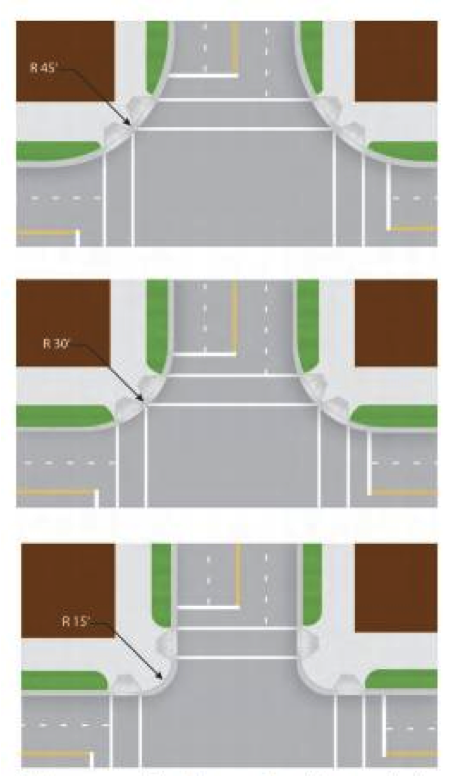
\includegraphics[scale=0.5]{location-depend.png}
	\caption{Different Curb Radii Depending on the Location}\label{fig:location-depend}
\end{figure}
	\subsection{third}
	\subsection{fourth}
	\subsection{fifth}
	\subsection{sixth}
	\subsection{seventh}
	\subsection{eighth}

\section{Analysis}
	\subsection{Methodology}
	\subsection{Rankings}
	\subsection{Discussion}

\section{Conclusion}

%description, impact, cost

\newpage

\nocite{*}
\bibliography{citations}{}
\bibliographystyle{plain}

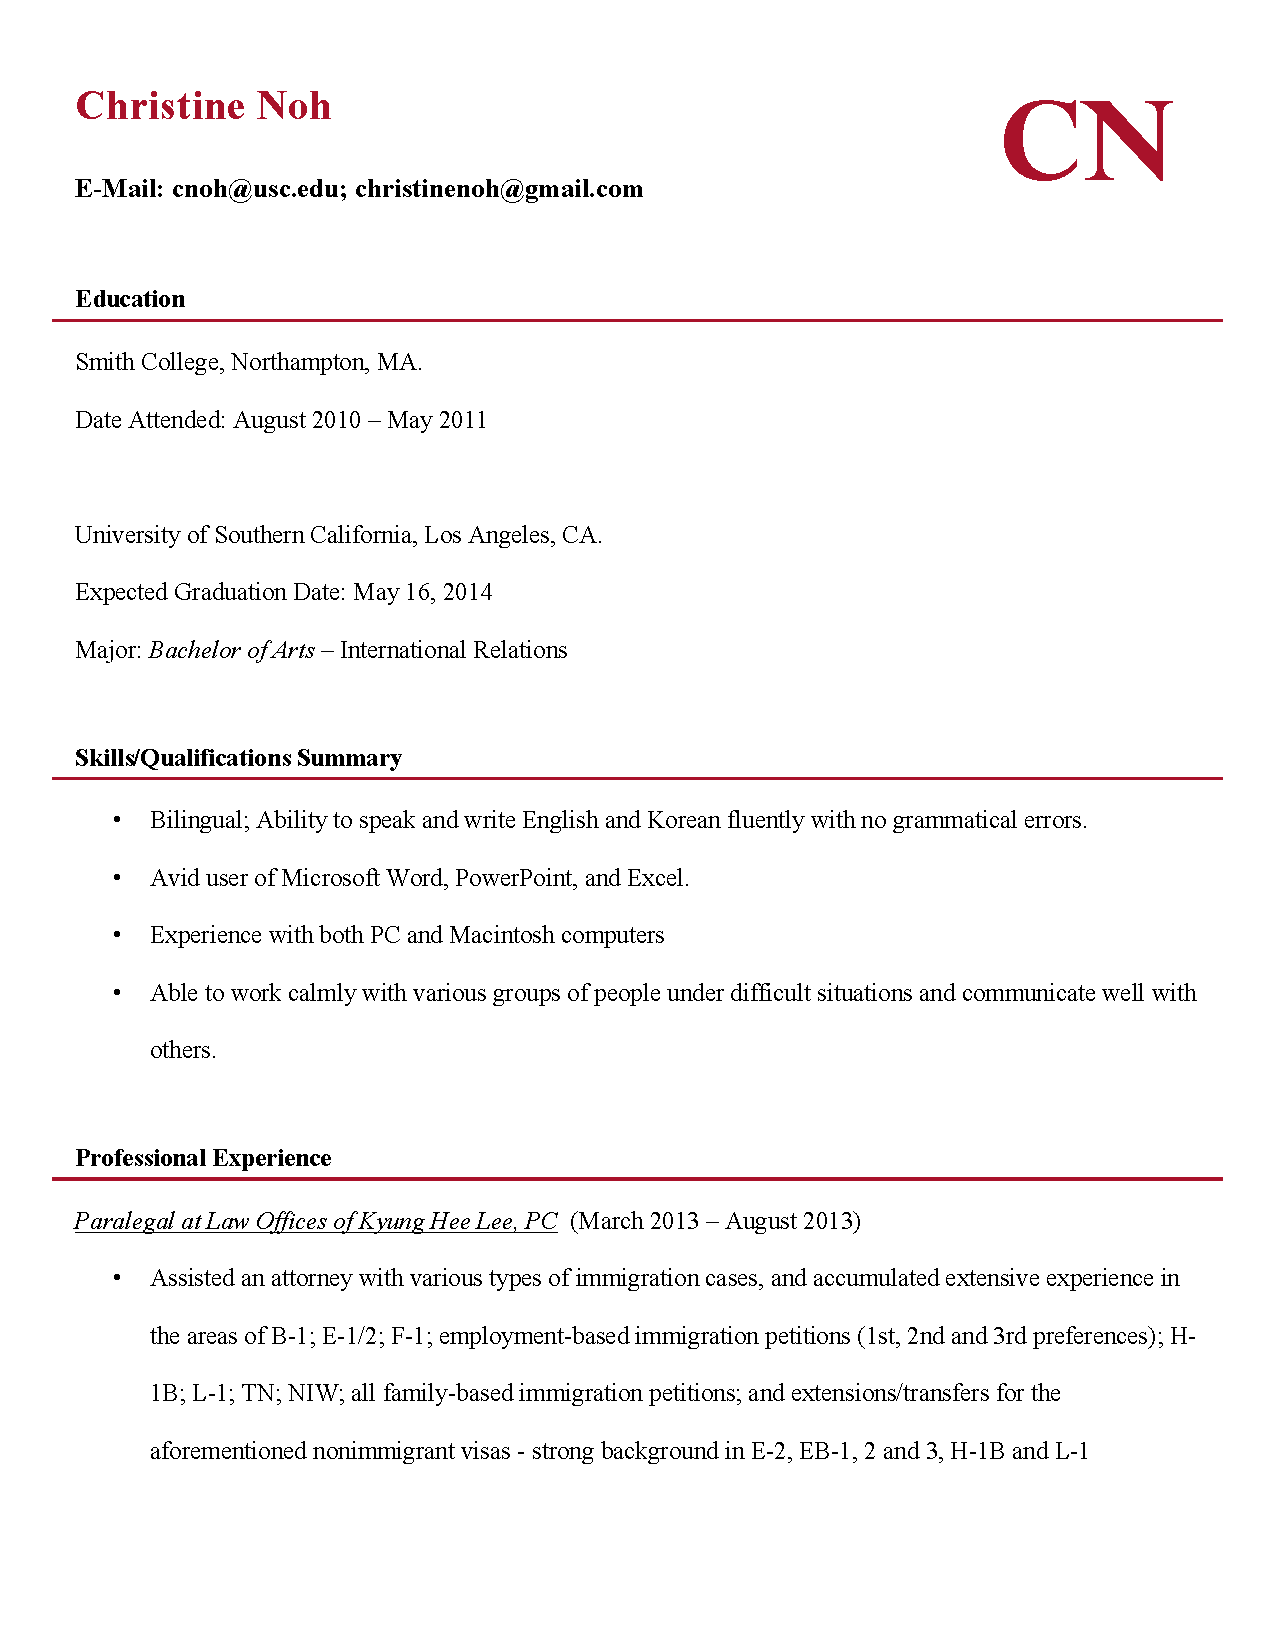
\includepdf{resumes/christine.pdf}


\end{document}